\section{Fundamentação Teórica}

\subsection{Aspectos de Engenharia de Software}

A importância de se projetar um software antes de implementá-lo é para que, mesmo que aumente a complexidade ou funcionalidades com o tempo, o software não seja comprometido a ponto dele não conseguir atingir todos os objetivos \cite{arqsoft}. A engenharia de software é, portanto, uma ferramenta para auxiliar desenvolvedores, incluindo técnicas de especificação, documentação, arquitetura e evolução de um programa. À medida que um programa evolui, ele precisa manter sua qualidade, que descreve como um software deve se comportar enquanto estiver executando e também descreve a estrutura e organização do sistema, associando esta descrição a uma documentação \cite{sommerville}.

Desta forma, o processo de criação de um software segue quatro passos bem definidos:
\begin{enumerate}

  \item Especificação ou Requisitos, o cliente e os desenvolvedores definem o software, bem como suas funcionalidades;
  \item Desenvolvimento, é feita a arquitetura do software e sua implementação;
  \item Validação, são aplicados testes para assegurar que os requisitos foram cumpridos;
  \item Evolução, o software é modificado de acordo com novas demandas do cliente.

\end{enumerate}

As mudanças rápidas de requisitos são uma consequência inevitável nos dias de hoje, tornando quase inviável a entrega de um software completamente funcional com todos os requisitos completos de uma única vez. Por conta disso, para equipes pequenas, opta-se por entregas incrementais, com pequenos intervalos de lançamento do software, e para cada lançamento um dos requisitos é implementado e validado. Este método de desenvolvimento é conhecido como método ágil \cite{sommerville}. Neste projeto, a metodologia ágil foi utilizada nos itens de desenvolvimento e de validação.

\subsubsection{Requisitos}

Requisito, na área de Engenharia de Software, pode ser definido como a especificação do que o software deve fazer, sendo um dos pilares no desenvolvimento de software \cite{sommerville}. Os requisitos refletem o que os usuários finais desejam que o programa deva realizar, podendo ser descritos tanto em alto nível de abstração (requisitos de usuário) ou descritos de forma mais detalhada que explica a nível de funcionamento de funções (requisitos do sistema). Além destes dois modos de descrever os requisitos, há ainda como classificá-los dependendo do que eles especificam. Se o requisito descrever o serviço que o sistema deve oferecer, explicando a resposta que ele deve fornecer ao usuário dada uma situação específica, e como deve ser seu comportamento em tempo de execução, este requisito é classificado como funcional. Se o requisito descrever as restrições do sistema, como tempo de desenvolvimento e tecnologia utilizada, então este requisito é classificado como não-funcional.

Para o levantamento de requisitos, podem ser aplicadas diversas formas de reunião com o cliente. Uma delas é o \emph{brainstorm}, quando as equipes se expressem individualmente sobre determinado assunto, sem restrições criativas e sem restrições quanto à exploração de opções, com o foco de quantidade ao invés de qualidade. Todas as ideias são anotadas e depois são analisadas pelo grupo \cite{brainstorm}. Só após a análise das ideias é que se descrevem os requisitos, seja da forma de requisitos do usuário ou da forma de requisitos do sistema \cite{sommerville}.

\subsubsection{Desenvolvimento}

Para aumentar modularidade e reusabilidade, funções de uso comum são incluídas em uma biblioteca. Uma biblioteca contém uma coleção de arquivos objetos, que podem ser ligados a um programa \cite{biblioteca}. Dada a documentação que explica as operações que serão oferecidas ao usuário, sua \acrfull{API} \cite{algoritmos}, sua implementação pode ser fornecida ao usuário de duas formas: estática ou dinâmica. 
Uma biblioteca estática é armazenada em disco, num arquivo de extensão \emph{.a} ou \emph{.lib}, o qual é concatenado ao arquivo executável que faz referência a funções da biblioteca. Já a ideia por trás de uma biblioteca dinâmica é ter apenas uma cópia das funções mais utilizadas armazenadas em memória, onde diferentes aplicações possam acessar as mesmas funções ao invés de cada uma ter sua própria cópia \cite{biblioteca}. Neste trabalho, optou-se por entregar aos usuários o projeto na forma de biblioteca dinâmica, onde o passo a passo da instalação da \playAPC{} está descrito no Guia de Referência (Apêndice \ref{appendix:guia}).

O paradigma orientado a objetos, usado neste projeto, utiliza o conceito de objetos para abstrair problemas. Um objeto é uma instância de uma classe que é criado e manipulado em tempo de execução. Apesar de se abstrair problemas utilizando o conceito de objetos, sua implementação é descrita por uma classe \cite{poo}. 

Classe é uma estrutura que possui atributos (variáveis de um objeto) e implementa métodos (funções de um objeto). Ela abstrai um conjunto de funcionalidades, ou seja, todos os seus atributos e métodos possuem relação com a característica que se deseja abstrair. Sub-classes são classes que herdam estas características, utilizando o princípio de herança. Herança define uma sub-classe hierarquicamente inferior que herda características de uma classe hierarquicamente superior \cite{poo}.

Neste trabalho, os problemas abstraídos foram os de computação gráfica, desta forma, laço de renderização, limpeza de \emph{buffer} ou detalhes de funcionamento da \acrshort{API} OpenGL~\cite{angel6th,cookbook,sb6,opengl8th,aot4} foram abstraídos e foi criada uma interface com estes elementos de computação gráfica. Esta interface é chamada de encapsulamento, no qual existem módulos bem definidos que realizam uma tarefa, sem o usuário necessariamente saber todas classes que foram utilizadas para a implementação desta tarefa \cite{poo}.

De modo a descentralizar uma grande aplicação, é viável a criação de um conjunto de classes que possam ter propósitos mais genéricos e que possam ser separadas em conjunto de funcionalidades, como uma camada que lida somente com a OpenGL, outra camada que lida somente com eventos, como entrada de teclado, criação de objetos, e uma última camada que cria uma interface amigável para o usuário. Desta forma, cada conjunto de classes presentes em uma camada são auto-suficientes e sua comunicação com outras camadas reduz-se a simples chamadas de métodos, definindo-se assim uma arquitetura em camadas. Com isso, aumenta a manutenabilidade do projeto~\cite{poo}. 

\subsubsection{Validação}

Testes apresentam tanto para os desenvolvedores quanto para os usuários o software por completo, assegurando que ele atingiu todos os requisitos, e também expõe comportamentos que não estavam previstos \cite{sommerville}. Para a verificação de ambos os casos, os testes são realizadas em duas etapas:
\begin{itemize}
\item Aplicar uma série de casos no programa para assegurar que ele funcione de modo esperado \cite{sommerville}.
\item Expor falhas do sistema que não necessariamente implicam em como o software será utilizado pelos usuários finais \cite{sommerville}. 
\end{itemize}


Neste projeto, optou-se por uma metologia de desenvolvimento de testes conhecida como \acrfull{TDD}. \acrshort{TDD} é um método que a cada nova implementação de função do software, é feito um teste para a função recém-implementada, e não são feitas novas implementações até esta ser aprovada \cite{sommerville}. Não foi utilizado nenhum \emph{framework} para a realização de testes, e sim foram criados programas simples, passando diferentes parâmetros para a função recém-implementada, onde se verificava se o resultado gráfico atendia o esperado. Alguns dos testes estão expostos no Guia de Referência, na parte de Documentação (Apêndice \ref{appendix:guia}).

\subsubsection{Evolução}

A evolução de um software é um processo que reflete as necessidades dos usuários finais, seja por meio de melhorias, novas funcionalidades ou uma crítica sobre um defeito que não foi detectado na etapa de validação. Estas necessidades devem refletir em novos requisitos, que vão passar por uma nova etapa de desenvolvimento, validação e assim entregue novamente aos usuários finais, repetindo indefinidamente este ciclo enquanto o software estiver ativo. Um bom software possui uma longa vida-útil \cite{sommerville}.

Neste projeto, para a avaliação de necessidade de alteração do comportamento das funções ou reformulação de algum dos requisitos, além de reuniões com professores interessados, foi proposto para o semestre 2016/2 a avaliação do projeto pelos alunos por meio de questionário de satisfação de uso. Este tipo de questionário é utilizado quando deseja-se avaliar um produto, caso este atenda as necessidades dos usuários finais e como eles o utilizam \cite{questionariodef}.

Um questionário de satisfação do cliente é um questionário fácil de apresentar, fácil de preencher e fácil de ser processado. Suas perguntas são relevantes ao produto, são concisas, não possui itens ambíguos, não são compostas e não possuem dupla-negativa \cite{questionariodef}. Para permitir várias respostas de graus diferentes, utiliza-se o método de resposta \emph{Likert}, em que são apresentadas múltiplas escolhas de respostas numa escala onde o participante pode concordar ou discordar em diferentes graus \cite{likert}.

Após a aplicação dos questionários, cada item pode ser avaliado separadamente e é feito o cálculo de média e a mediana nos itens que se utilizou o método \emph{Likert} \cite{likert}, tendo um balanço geral do produto no período pesquisado.


\subsection{Aspectos de Computação Gráfica}

A computação gráfica é uma comunicação visual por meio da tela do computador, tanto no sentido computador-humano quanto no sentido humano-computador. É uma área multidisciplinar que envolve física, matemática, percepção humana, engenharia e arte: física para modelar a luz e realizar simulações, matemática para descrever as formas geométricas, engenharia para otimizar tempo de uso de processor e memória e arte combinada com percepção humana para deixar esta comunicação mais efetiva \cite{cgintro}.

\begin{figure}
  \centering
  \begin{subfigure}[t]{.8\textwidth}
    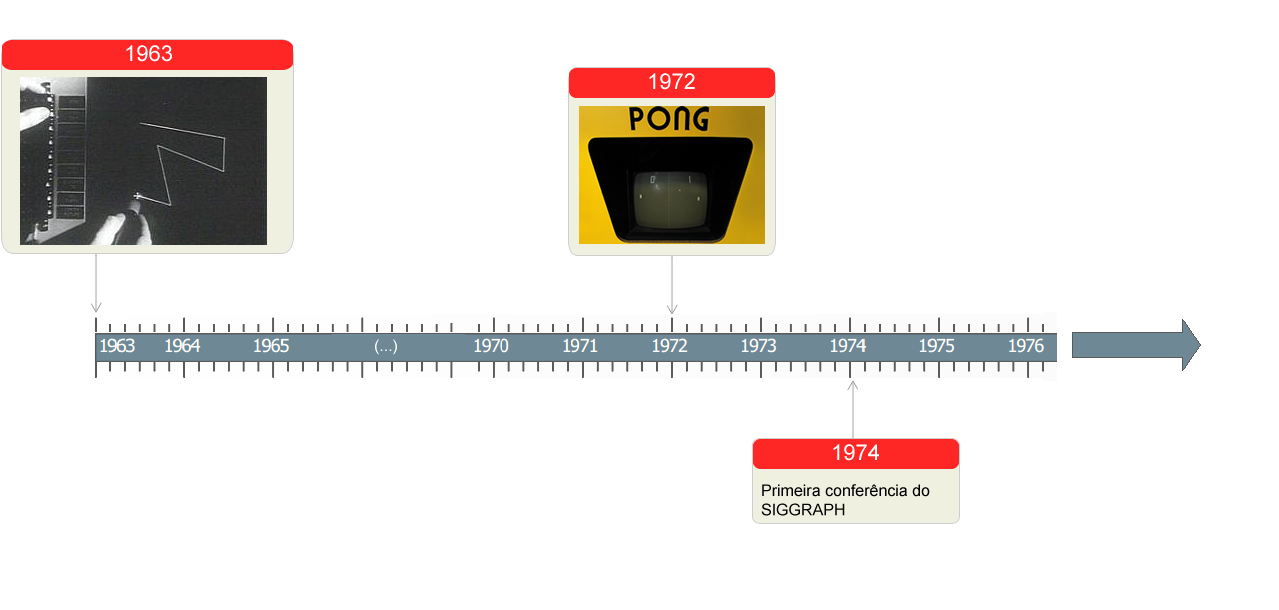
\includegraphics[scale=0.4]{img/timeline1}
    \caption{1963 à 1976.} 
  \end{subfigure}
  ~
  \begin{subfigure}[t]{.8\textwidth}
    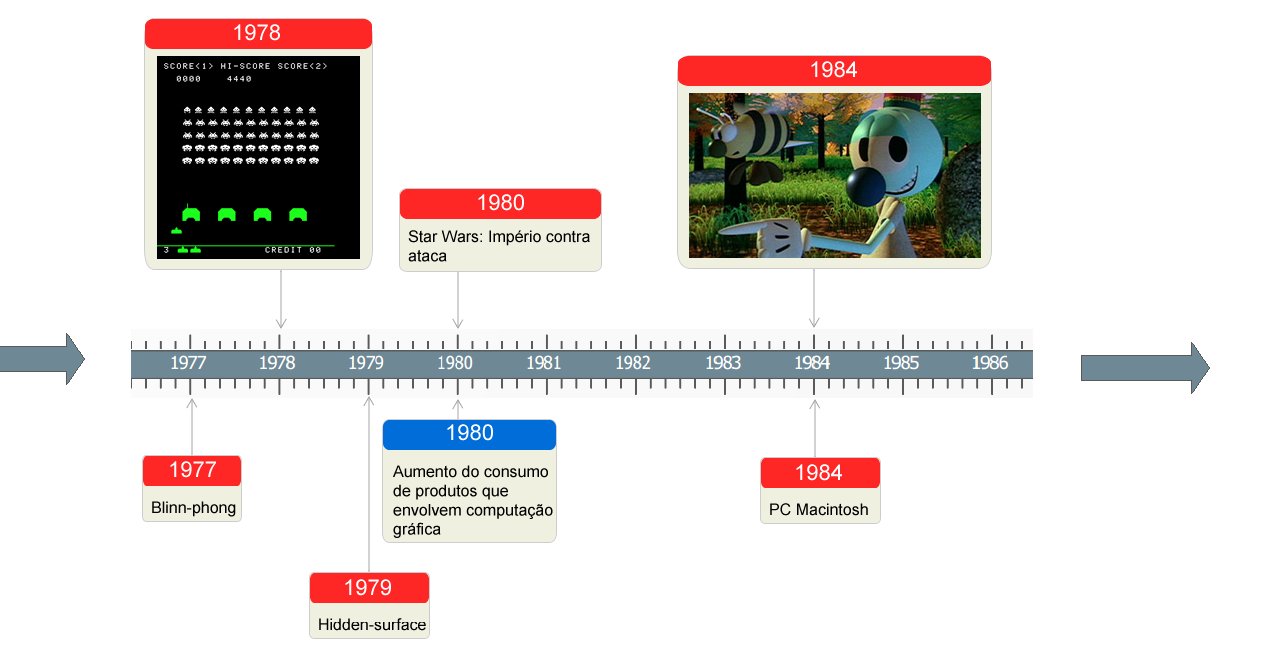
\includegraphics[scale=0.4]{img/timeline2}
    \caption{1977 à 1986.} 
  \end{subfigure}
  ~
  \begin{subfigure}[t]{.8\textwidth}
    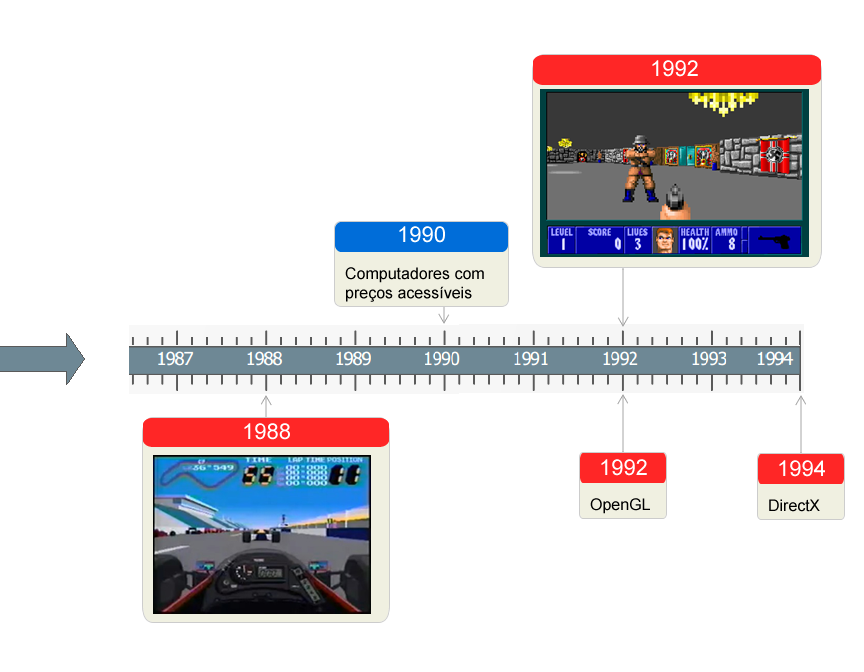
\includegraphics[scale=0.4]{img/timeline3}
    \caption{1987 à 1994.} 
  \end{subfigure}

  \caption{Linha do tempo resumida da Computação Gráfica: a) Anos 60 à anos 70; b) Anos 70 à anos 80; c) Anos 80 à anos 90;} \label{fig:timeline}
\end{figure}

O estudo nessa área se iniciou por volta de 1963, com o Ivan Sutherland, que implementou o primeiro programa que utilizava uma interface gráfica, o Sketchpad. Sketchpad recebia do usuário pontos $x$ e $y$ em sua tela e exibia vetores ligando esses pontos, demonstrando o uso da computação de forma artística e técnica. O Sketchpad usava o computador Lincoln TX-2, desenvolvido especificamente para o primeiro Sketchpad \cite{sketchpad}. 

 % \begin{savenotes}
 % \begin{figure}[H]
 %     \centerline{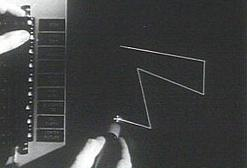
\includegraphics[width=.5\textwidth]{img/sketchpad}}
 %     %\caption{Programa Sketchpad \footnote{\url{http://www.nakedobjects.org/book/section5.html}}.}
 %     \caption{Programa Sketchpad \footnote{teste}.}
 %     \label{fig:sket}
 %   \end{figure}
 % \end{savenotes}

 \begin{figure}[H]
    \centering
    \centerline{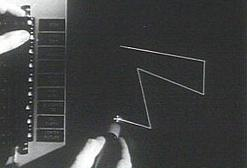
\includegraphics[width=.5\textwidth]{img/sketchpad}}
    \caption{Exemplo de computação gráfica em 1960: Programa Sketchpad \protect\footnotemark.}
\end{figure}
\footnotetext{Fonte: \url{http://www.nakedobjects.org/book/section5.html}}

No final desta década, criou-se o grupo especial interessados em computação gráfica, \emph{Special Interest Group on Computer Graphics} (SIGGRAPH), que organizava conferências, determinava padrões e publicava artigos dentro da área de computação gráfica, cuja a primeira conferência foi realizada em 1974 \cite{siggraph}. Também naquele período, iniciou-se a produção de jogos eletrônicos utilizando \emph{sprites} 2D, que são imagens bidimensionais que se movimentam na tela\cite{sprite}. Exemplos de jogos desta época foram o \emph{Pong}, sendo o primeiro jogo comercial em fliperamas em 1972 \cite{pong}, e \emph{Space Invaders} em 1978, sendo um dos primeiros jogos a utilizar uma grande quantidade de \emph{sprites}  na tela e precusor da importância da temática de um jogo \cite{intrgames}. Ambos os jogos utilizavam o controlador de vídeo \emph{Fujitsu} MB14241, especializado em criação e renderização de \emph{sprites} 2D \cite{fujitsu}, sendo renderização definida como processo que o computador utiliza para criar uma imagem dado um modelo \cite{opengl8th}. 
Paralelamente, na Universidade de Utah, um grupo de pesquisadores avançavam a pesquisa para o campo 3D, estudando como determinar qual objeto está na frente ou atrás do espectador, iniciando os estudos de algoritmos de  \emph{hidden-surface} \cite{hidden}, e como o objeto teria um aspecto de volume, iniciando os estudos de sombreamento no próprio objeto,  como o algortimo de sombreamento de Blinn-Phong \cite{phong}.

\begin{savenotes}
 \begin{figure*}[!htp]
    \centering
    \begin{subfigure}[t]{0.4\textwidth}
        \centerline{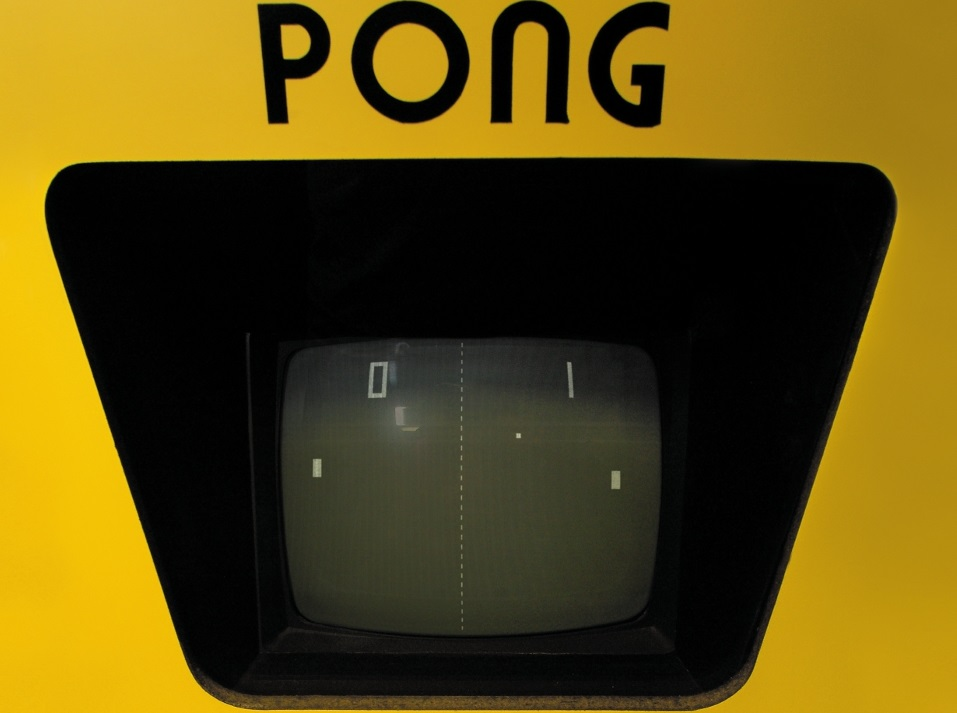
\includegraphics[width=.9\textwidth]{img/pong1}}
        \caption{Jogo Pong \footnote{Fonte: \url{https://todayinhistoryblog.wordpress.com/tag/pong/}}.}
    \end{subfigure}
    ~
    \begin{subfigure}[t]{0.4\textwidth}
        \centerline{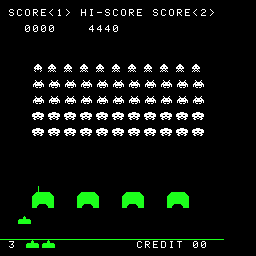
\includegraphics[width=.9\textwidth]{img/si}}
        \caption{Jogo Space Invaders \footnote{Fonte: \url{http://www.brentradio.com/SpaceInvaders.htm}}.}
    \end{subfigure}
    \caption{Exemplo de computação gráfica em 1970: a) Jogo Pong; b) Jogo Space Invaders.}

\end{figure*}
\end{savenotes}


A partir dos anos 1980, a necessidade de desenvolvedores gráficos aumentou drasticamente e isso se refletiu nos produtos comercializados à época. Entre os mais populares, o computador pessoal Macintosh, que popularizou e padronizou o uso de interface gráfica para usuários \cite{macintosh}; o segundo filme da trilogia original de \emph{Star Wars}, com o avanço na utilização da técnica \emph{chroma-key} pela empresa Lucasfilm \cite{chromakey}; milhares de cópias de jogos para Atari, Sega e Nintendo foram vendidos \cite{intrgames}, enquanto nos fliperamas começavam a utilizar as primeiras placas gráficas dedicadas para renderização 3D, como a \emph{Namco System 21} \cite{fujitsu} para o jogo \emph{Winning run} \cite{videogamebum}; e o primeiro curta metragem totalmente gerado por computador, o \emph{The Adventures of André and Wally B.}, desenvolvido pela Pixar, que iniciou o estudo na área de \emph{shaders} \cite{curtapixar}, programas que realizam ajuste no nível de cores em objetos 3D.

\begin{savenotes}
 \begin{figure}[H]
    \centering
    \begin{subfigure}[t]{0.5\textwidth}
        \centerline{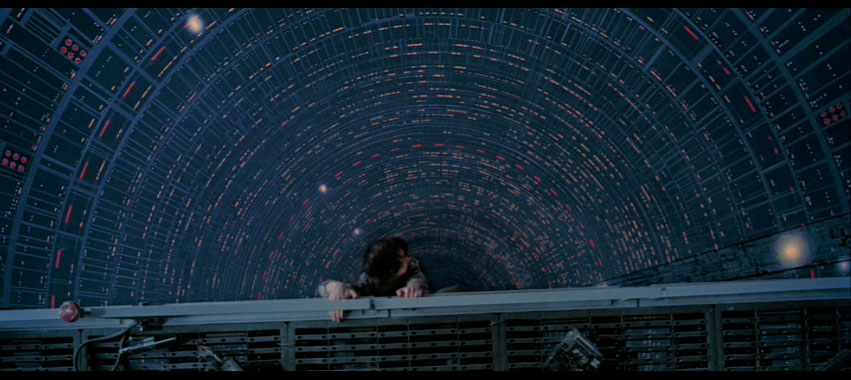
\includegraphics[width=.9\textwidth]{img/starwars}}
        \caption{Cena do filme Star Wars episódio V - O império contra ataca \footnote{Fonte: \url{https://kharisampson.wordpress.com/tag/star-wars/}}.}
    \end{subfigure}
    ~
    \begin{subfigure}[t]{0.3\textwidth}
        \centerline{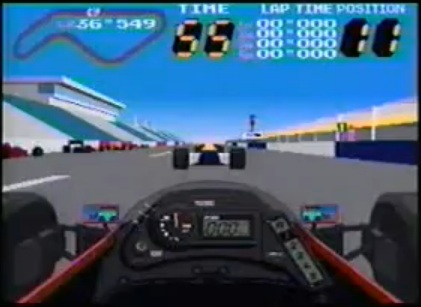
\includegraphics[width=.9\textwidth]{img/winning_run}}
        \caption{Jogo Winning Run \footnote{Fonte: \url{http://www.gamespot.com/forums/games-discussion-1000000/evolution-of-video-game-graphics-29361008/}.}}
    \end{subfigure}
    ~
    \begin{subfigure}[t]{0.3\textwidth}
        \centerline{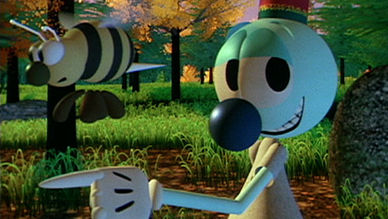
\includegraphics[width=.9\textwidth]{img/curtapixar}}
        \caption{Cena do curta \emph{The Adventures of André and Wally B.} \footnote{Fonte: \url{http://pixaranimationshorts.wikia.com/wiki/The_Adventures_Of_Andre_and_Wally_B}}}
    \end{subfigure}

    \caption{Exemplo de computação gráfica em 1980: a) Filme Star Wars; b) Jogo Winning Run; c) Curta \emph{The Adventures of André and Wally B.}.}

\end{figure}
\end{savenotes}


Em 1990, à medida que os computadores pessoais aumentavam sua capacidade de processamento a preços mais acessíveis \cite{evopc}, surgiu a necessidade de padronizar processamento gráficos e quais seriam os padrões de projeto adotados pelos desenvolvedores de hardwares e de softwares gráficos. A primeira geração de \acrfull{GPU} renderizava somente um \emph{pixel} por ciclo de \emph{clock}, implicando que a \emph{CPU} enviada mais informação que a \acrshort{GPU} conseguia processar, como por exemplo o RIVA TNT, da empresa Nvidia \cite{nvidia}. Ainda assim, nesta época foram lançados jogos que se utilizavam desta nova tecnologia, como Wolfenstein 3D em 1992 \cite{videogamebum}. Apenas anos mais tarde foram adicionados \emph{pipelines} e núcleos na \acrshort{GPU} para estes \emph{pixels} serem processados paralelamente \cite{nvidia}.
%Em 1999, a empresa \emph{Nvidia} lançou o primeiro processador gráfico para computadores pessoais capaz de realizar cálculos de transformações matriciais, realizar cálculos para iluminação e sombreamento de objetos e possuía uma \emph{engine} de renderização, seja para objetos 3D ou 2D, a \acrfull{GPU} GeForce 256 \cite{nvidia}. 

 \begin{figure}[H]
    \centering
    \centerline{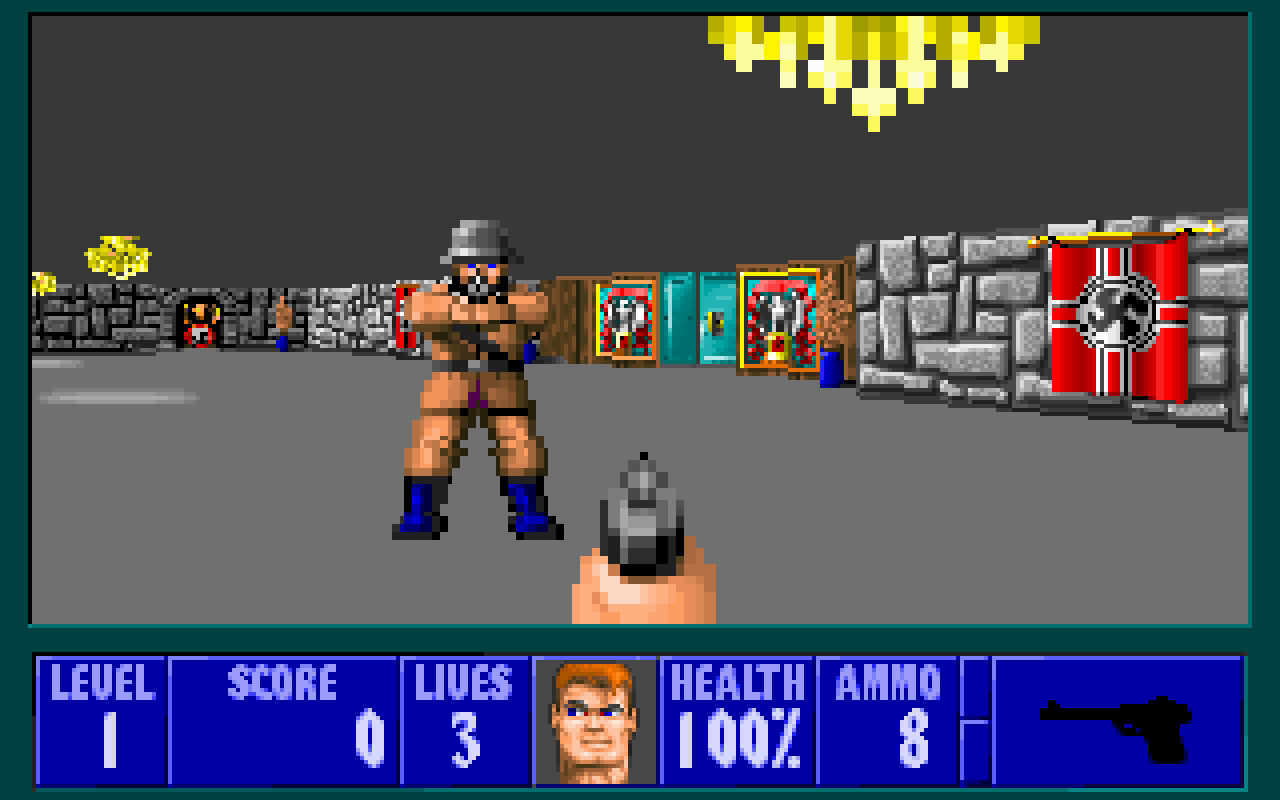
\includegraphics[width=.5\textwidth]{img/wolfenstein}}
    \caption{Exemplo de computação gráfica em 1990: Jogo Wolfenstein 3D \protect\footnotemark.}
\end{figure}
\footnotetext{Fonte: \url{https://3drealms.com/catalog/wolfenstein-3d_25/}}


Para padronizar o uso dos recursos das \acrshort{GPU} que estavam sendo lançadas, foram criadas duas \acrshort{API} naquela época, a DirectX, lançado em 1994 exclusivamente feito para plataformas Windows, e a OpenGL, lançada em 1992 para diversas as plataformas \cite{apigpu}. A \acrshort{API} DirectX lida não apenas com renderização de objetos 3D, mas também gerencia som, entrada de dispositivos e comunicação entre redes \cite{openglgame}. A OpenGL assume que a alocação de memória responsável pela exibição de \emph{pixels} na tela seja feita pelo sistema operacional, ou seja, ela é responsável somente pela atualização do \emph{buffer} de memória gráfico, mais especificamente, o \emph{Frame Buffer} \cite{johnnyartigo}, o que garante sua portabilidade \cite{CG2D}. 

Devido a sua proposta multiplataforma, a OpenGL possui inúmeras aplicações\footnote{\url{https://www.opengl.org/news/categories/C3}}, como interfaces gráficas para aplicações diversas e jogos tanto para consoles quanto para computadores, é aplicada em diferentes linguagens de programação, como C/C++, Java, ADA, Python, Fortran e Perl, e está em constante atualização e reformulação, sendo a mais recente conhecida como Vulkan \cite{vulkan}, uma versão mais flexível da OpenGL 4.5 e compatível com dispositivos mais modernos. Por isso, a OpenGL tornou-se parte indispensável do \emph{design} de grande parte dos hardwares gráficos \cite{nvidia}.

As primeiras \acrshort{GPU} possuíam a arquitetura conhecida como \emph{pipeline} fixo: quando os programadores enviavam dados para \acrshort{GPU}, os dados não poderiam ser modificados \cite{nvidia}. A Figura \ref{fig:arqopengl} exibe a arquitetura do \emph{pipeline} fixo utilizando exemplos de funções da OpenGL. 

 \begin{figure}[H]
    \centering
    \centerline{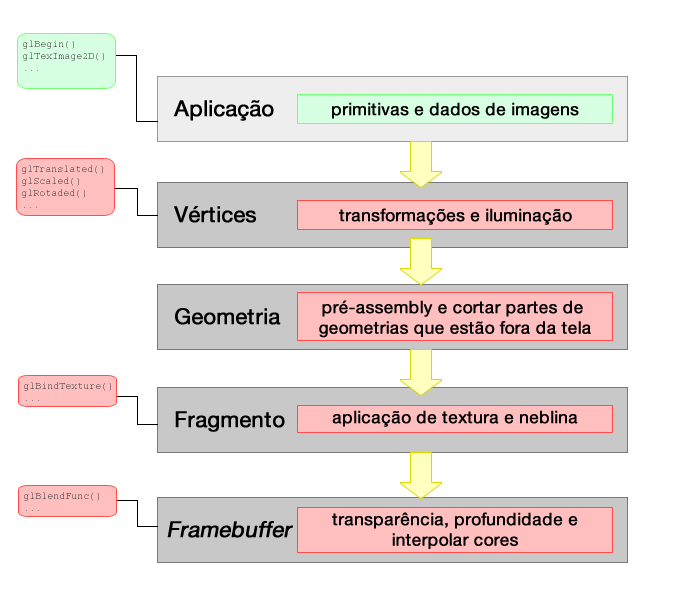
\includegraphics[width=1.3\textwidth]{img/opengl2}}
    \caption{Representação gráfica do \emph{pipeline} fixo\protect\footnotemark. Em verde, estágio do \emph{pipeline} em que o programador tem acesso direto; em vermelho, estágios do \emph{pipeline} que o programador não tem acesso direto e precisa utilizar funções pré-definidas que precisam sempre passar pelo nível de aplicação até atingir o nível que ela é executada. Os balões nos estágios do \emph{pipeline} exemplificam funções que só executam naquele nível.}
    \label{fig:arqopengl}
\end{figure}
\footnotetext{Adaptado de: \url{https://developer.apple.com/library/content/documentation/GraphicsImaging/Conceptual/OpenGL-MacProgGuide/opengl_shaders/opengl_shaders.html}}


Para acompanhar esta arquitetura, as \acrshort{API} definiam o método de programação conhecido como modo imediato, os dados que seriam processados pela \acrshort{GPU} só eram enviados no momento de execução do programa \cite{imediato}. 

Anos mais tarde, este método mostrou-se extremamente ineficiente \cite{learnopengl}, pois a \acrshort{GPU} passa um tempo considerável de forma ociosa \cite{opengl3th}. Somente a partir de 2002 que as \acrshort{GPU} permitiram que programadores utilizassem \emph{shaders} em suas aplicações, modificando os dados enviados para \acrshort{GPU} em diferentes estágios do \emph{pipeline} \cite{nvidia}. Esta mudança de paradigma refletiu na versão 2.0 da OpengGL, que descontinuou o modo imediato.

Como a computação gráfica é uma área relativamente nova e em constante atualização, consideramos neste trabalho que o público alvo tem acesso, a pelo menos, placas de vídeos com \emph{pipeline} fixo, compatível com a versão 1.3 da OpenGL. Nesta versão, como a OpenGL disponibiliza apenas funções de baixo nível, tratando-se diretamente com o driver OpenGL da placa de vídeo, optou-se por utilizar a biblioteca GLU, \emph{OpenGL Utility Toolkit}, que possui um conjunto de funções de alto nível, como implementações de transformações lineares, mapeamento da tela e algumas primitivas geométricas \cite{glu}.  

Há diversos tipos de biblioteca que podem ser utilizadas em conjunto com a OpenGL que facilitam o seu uso. Neste projeto, optou-se por utilizar uma biblioteca para o gerenciamento da janela que são renderizadas cenas utilizando OpenGL e outra biblioteca para o mapeamento de textura \cite{angel6th}, que utiliza uma imagem, vetor de \emph{pixels}, para influenciar a cor do fragmento no ponto da superfície do polígono.
A GLFW 2.7 é uma API específica para o uso com a OpenGL feita com a linguagem C. Sua proposta é, além de facilitar o gerenciamento de uma janela de contexto, inclui as seguintes funcionalidades:
\begin{itemize}
  \item entrada de teclado, mouse e joystick
  \item maior precisão de tempo
  \item suporte a \emph{mult-threading}
  \item suporte de \emph{query} e uso de extensões da OpenGL
  \item suporte básico de carregamento de imagens
\end{itemize}
SOIL é uma biblioteca feita em C que é usada para carregar texturas usando OpenGL, com a proposta de ser simples e multi-plataforma. Ela consegue ler imagens no formato BMP, JPG, PNG, TGA, DDS, PSD e HDR, carregando as imagens diretamente como texturas \cite{SOIL}.

\subsubsection{Aspectos Técnicos da OpenGL}

Os modelos renderizados pela OpenGL são construídos com formas geométricas primitivas, como ponto, linha e triângulo, sendo eles definidos pelos seus vértices, representados da forma $p = (x, y, z)$ ou da forma matricial 
$
  p = \begin{bmatrix}
  x\\ 
  y\\ 
  z
  \end{bmatrix}
$ \cite{opengl8th, angel6th}. 
Devido a esta forma de representação das primitivas, as operações realizadas pela OpenGL seguem definições da Álgebra linear, que é uma área da matemática derivada da geometria analítica no plano e espaço e busca a resolução de sistemas lineares \cite{labma}. 

Um dos conceitos essenciais para a computação gráfica é que as operações possíveis são feitas dentro de um espaço vetorial, que é definido por:
\begin{itemize}
  \item um conjunto não vazio $V$, cujo os elementos são chamados de vetores
  \item conjunto numérico $K$, cujo elementos são chamados de escalares
  \item uma soma vetorial: operação que associa a cada dois vetores $ v, u \in V $ um vetor $ v + u \in V $
  \item uma multiplicação por escalar: operação que associa a cada vetor $v \in V$ e um escalar $k \in K$ um vetor $kv \in V$
\end{itemize}

Tipicamente, haverão diversas geometrias em posições específicas em uma cena. Quando deseja-se modificar estas geometrias, é necessário utilizar transformações lineares para modificar suas posições originais \cite{opengl8th}.
Seja $V$ e $W$ dois espaços vetorais, define-se \cite{alT} uma função de transformação linear $T$ como:
  \begin{equation*}
      T:V \rightarrow W
  \end{equation*}
Para cada elemento $v \in V$ e $w \in W$ teremos:
  \begin{equation*}
      w = T(v)
  \end{equation*}
% Dada as limitações da versão da OpenGL e do plano 2D da \playAPC, foram utilizadas três transfomações lineares: translação, rotação e redimensionamento.

\paragraph{Translação} \mbox{}\\
Translação é um deslocamento de um ponto a outro ponto em um plano. Dado o vetor de deslocamento $d$, calcula-se para todos os pontos da figura sua translação pela Equação \ref{eq:translada} ~\cite{angel6th}.
  \begin{equation} \label{eq:translada}
      T(v) = v + d
  \end{equation}

\begin{figure}[H]
  \centering
  \begin{subfigure}[t]{.25\textwidth}
    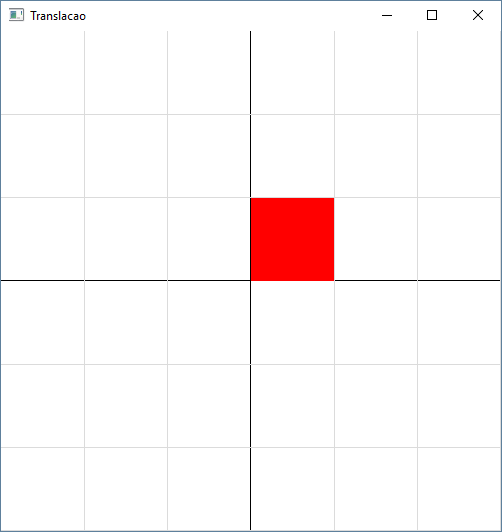
\includegraphics[width=.9\textwidth]{img/linear1a}
    \caption{Figura na posição original.} 
  \end{subfigure}
  ~
  \begin{subfigure}[t]{0.25\textwidth}
    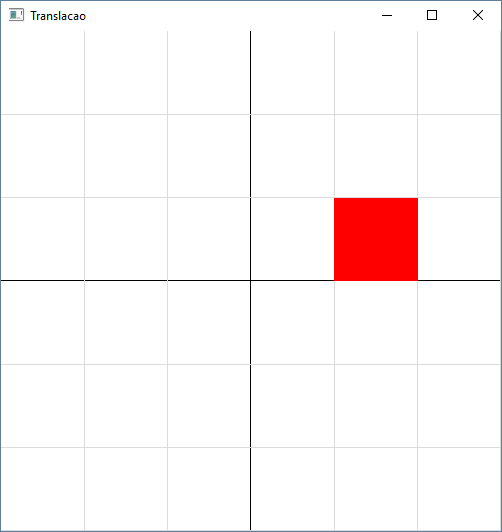
\includegraphics[width=.9\textwidth]{img/linear1b}
    \caption{Figura na posição transladada em 10 unidades.} 
  \end{subfigure}
  \label{fig:linear1}
  \caption{Translação: a) Posição original; b) Transladado.} 
\end{figure}

\paragraph{Rotação} \mbox{}\\
Dado um ângulo $\Theta$, rotaciona-se a figura em torno da origem do sistema. Um ponto particular $(x,y)$ será rotacionado para a posição $(x',y')$ dado um ângulo $\Theta$. Este cálculo é feito como ilustra a Equação \ref{eq:rot} \cite{angel6th}.
  \begin{equation} \label{eq:rot}
      \begin{bmatrix}
      x'\\ 
      y'
    \end{bmatrix} 
    = 
    \begin{bmatrix}
      cos\Theta  & -sin\Theta \\ 
      sin\Theta& cos\Theta
    \end{bmatrix}
    \begin{bmatrix}
      x\\ 
      y
    \end{bmatrix}
  \end{equation}

  \begin{figure}[H]
  \centering
  \begin{subfigure}{.25\textwidth}
    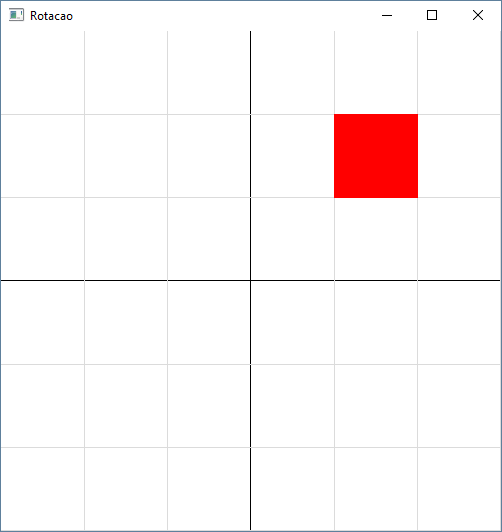
\includegraphics[width=.9\textwidth]{img/linear2a}
    \caption{Figura na posição original.} 
  \end{subfigure}
  ~
  \begin{subfigure}{.25\textwidth}
    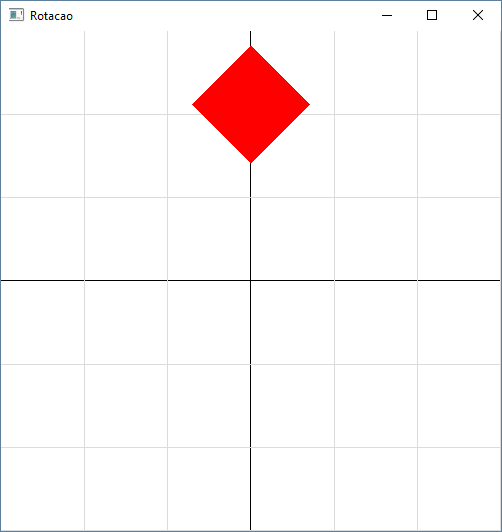
\includegraphics[width=.9\textwidth]{img/linear2b}
    \caption{Figura na posição rotacionada em 45 graus.} 
  \end{subfigure}
  ~
  \begin{subfigure}{.25\textwidth}
    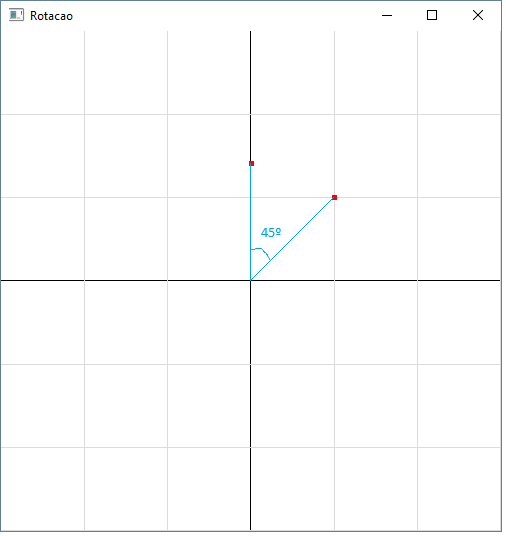
\includegraphics[width=.9\textwidth]{img/linear2c}
    \caption{Ponto rotacionado em 45 graus.} 
  \end{subfigure}
\label{fig:linear2}
\caption{Rotação: a) Posição original; b) Quadrado rotacionado; c) Ponto rotacionado.} 
\end{figure}

\paragraph{Escala} \mbox{}\\
Escala é uma transformação aplicada em um corpo não uniforme, que o faz maior ou menor. Dada quatro constantes $\alpha_x$, $\alpha_y$, $\alpha_z$ e $\alpha_w$, sendo $\alpha_w = 1$ , o cálculo de sua transformação de escala, para cada ponto, é feito como ilustra a Equação \ref{eq:esc} \cite{opengl8th}.
\begin{equation} \label{eq:esc}
  \begin{bmatrix}
      x'\\ 
      y' \\
      z' \\
      1
    \end{bmatrix} 
    = 
    \begin{bmatrix}
     \alpha_x& 0 & 0 & 0 \\ 
     0 & \alpha_y & 0 & 0\\ 
     0& 0 & \alpha_z & 0\\ 
     0& 0 & 0 & 1
  \end{bmatrix}
  \begin{bmatrix}
      x\\ 
      y\\
      z\\
      w\\
    \end{bmatrix}
\end{equation}

Para o caso de manipulação de objetos em duas dimensões, os termos $z'$, $\alpha_z$, $z$ e são iguais a $1$.
  
\begin{figure}[H]
  \centering
  \begin{subfigure}[t]{.25\textwidth}
    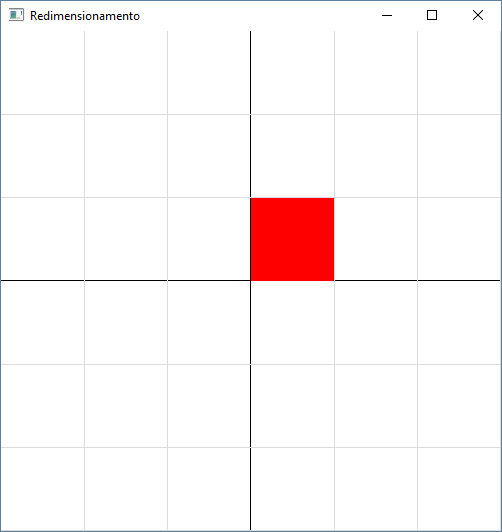
\includegraphics[width=.9\textwidth]{img/linear3a}
    \caption{Figura original.} 
  \end{subfigure}
  ~
  \begin{subfigure}[t]{.25\textwidth}
    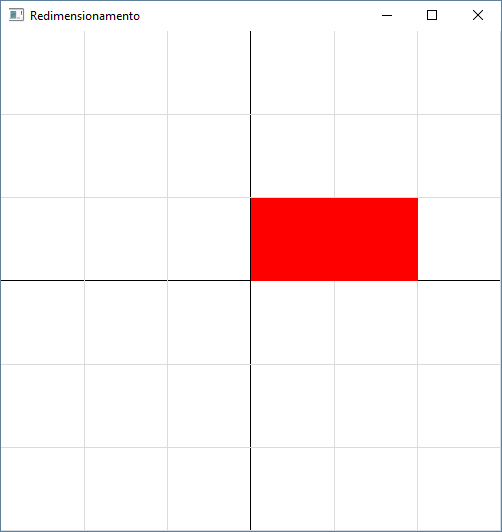
\includegraphics[width=.9\textwidth]{img/linear3b}
    \caption{Figura redimensionada em dobro no eixo x.} 
  \end{subfigure}
  ~
  \begin{subfigure}[t]{.25\textwidth}
    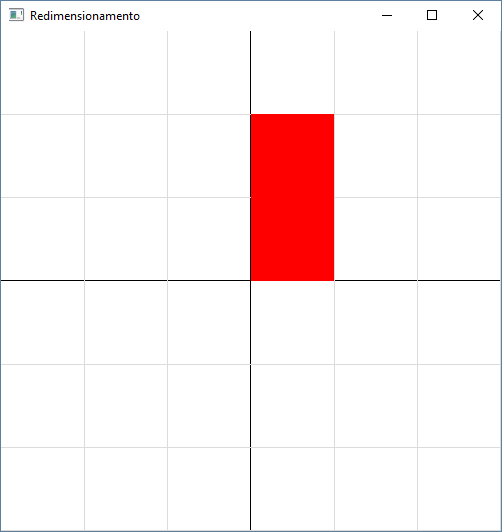
\includegraphics[width=.9\textwidth]{img/linear3c}
    \caption{Figura redimensionada em dobro no eixo y.} 
  \end{subfigure}
  \label{fig:linear3}
  \caption{Redimensionamento: a) Figura original; b) $\alpha_x = 2$, $\alpha_y = 1$; c) $\alpha_x = 1$, $\alpha_y = 2$.} 
\end{figure} 



%O mercado também se adaptou a esta demanda distribuindo cada vez melhores e mais potentes placas de vídeos \emph{GPU}, otimizadas para renderização de objetos 2D e 3D na tela, apesar de também estar sendo utilizada em aplicações de alto desempenho \cite{gpu}.

% \paragraph{OpenGL}
% OpenGL é uma API para renderizar gráficos 3D utilizando procedimentos específicos do \emph{hardware} dedicado para este processo, a placa de vídeo (\emph{GPU}), sendo a renderização do 2D apenas um caso particular do 3D. A Figura ~\ref{fig:arqopengl} ilustra a arquitetura da OpenGL, exibindo a comunicação da \emph{CPU} e \emph{GPU}~\cite{johnnyartigo}. 


% A OpenGL assume que a alocação de memória responsável pela exibição de \emph{pixels} na tela seja feita pelo sistema operacional, garantindo sua portabilidade \cite{CG2D} para inúmeros sistemas, sendo somente responsável pela atualização do \emph{buffer} de memória gráfico, mais especificamente, o \emph{Frame Buffer} \cite{johnnyartigo}.

% \subparagraph{Modo Imediato}
% O modo imediato da OpenGL é um modo de renderização descontinuado desde a versão 2.0 da OpenGL, até torna-se deprecado a partir da versão 3.0, tornando-se um modo legado. Neste modo, a CPU informa quais objetos serão renderizados pela GPU no momento de execução do programa \cite{imediato}, resultando num processo de renderização menos eficiente \cite{learnopengl}, pois haverá muitos momentos que a GPU estará ociosa esperando o fluxo do programa indicar quando ela deverá ser acionada  \cite{opengl3th}.

\paragraph{Visualização} \mbox{}\\

Se exibirmos modelos geométricos utilizando diretamente as coordenadas da tela do computador, provavelmente as coordenadas do modelo não estariam na mesma proporção que as coordenadas da tela, devido a diferença de alcance de ambos os sistemas. Desta forma, utilizamos transformações nas matrizes relacionadas a visualização para ajustar o sistema de coordenadas de ambos, projetando o modelo de forma coerente na tela \cite{opengl8th}.

%O processo para produzir a visualização desejável na janela é análogo ao de tirar uma foto, como ilustra a Figura \ref{fig:camera}.
% \begin{figure}[h!]
%   \begin{center}
%     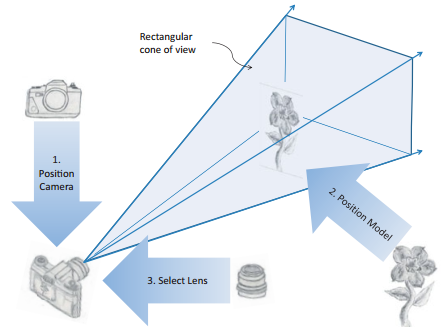
\includegraphics[scale=0.8]{img/camera}
%   \end{center}
%   \caption{Analogia da câmera da OpenGL e uma câmera real, do livro \emph{OpenGL Programming Guide}, página 207 \cite{opengl8th}. }
%   \label{fig:camera}
% \end{figure}


O processo para produzir a visualização 2D de uma cena 3D na janela é análogo ao de tirar uma foto. Enumerando os passos para tirar a foto, devemos:
\begin{enumerate}
  \item Ajustar a posição da câmera, com as lentes apontando para o local desejado (transformações na Matriz de \emph{viewing}, matriz responsável pela orientação do sistema e volume de alcance da renderização);
  \item Mover o objeto para posição desejada (transformações do modelo: translação, rotação, redimensionamento);
  \item Escolher a lente e ajustar o zoom (transformações nas Matrizes de Projeção, matriz responsável pela manipulação de coordenadas, se o objeto estará próximo ou distante de algum ponto de referência);
  \item Tirar a foto (aplicar transformações) e;
  \item Escolher tamanho da foto (transformações na Matriz de \emph{viewport}, matriz responsável pela conversão de coordenadas do sistema para coordenadas da janela);
\end{enumerate}

Para a visualização de um sistema 2D \cite{CG2D}, que é um caso particular do 3D, é necessário ajustar somente a Matriz de Projeção Ortogonal. Esta matriz indica que um dos eixos não será utilizado (normalmente o eixo $z$), mantendo o valor de $-1$ e $1$ para seus limites, portanto não há perspectiva. Ela é ajustada determinando os limites dos eixos $x$ e $y$, sendo necessário também calcular o aspecto da visualização de acordo com o tamanho em $pixel$ da janela de visualização.

% \paragraph{GLU}
% GLU \emph{OpenGL Utility Library} é uma biblioteca que cria uma interface com a OpenGL. Ela possui um conjunto de funções de alto nível, como por exemplo transformações lineares, mapeamento da tela e algumas primitivas geométricas, sendo estas funções compatíveis com a versão 1.3 da OpenGL~\cite{glu}.


\subsection{Aspectos Educacionais}

Educação é um conjunto de normas que desenvolvem hábitos, costumes e valores de uma sociedade, ou seja, é um processo contínuo de desenvolvimento das faculdades físicas, intelectuais e morais do ser humano. Em estabelecimentos de ensino, a educação é entregue aos indivíduos com intuito de desenvolver o raciocínio lógico e crítico dos alunos. O modelo predominantemente empregado nestes estabelecimentos é o modelo expositivo, o ensino está centrado no professor e o aluno transcreve nas avaliações o conhecimento adquirido pelos professores \cite{educacao}. Entretanto, segundo o Dr. em Psicologia Social Douglas Tavares Borges Leal: 
\say{A aula expositiva caracteriza-se pela autoridade do professor diante de seu aluno, provocando sérios problemas de comunicação}.
O Dr. também afirma que: 
\say{O conteúdo a ser aprendido é apresentado ao aprendiz na sua forma final e a tarefa da aprendizagem não envolve nenhuma descoberta independente por parte do estudante}.
Questiona-se, então, a qualidade de informação que o aluno absorve, uma vez que não é medido a capacidade crítica do aluno, e sim a capacidade de replicar informação \cite{expositivo}. 

Nos cursos de computação, mesmo sendo uma área em constante atualização, também é aplicado esta metodologia de ensino. Devido a restrições deste método, observa-se que os principais problemas no ensino de programação são \cite{ludicoalgoritmo}:
\begin{itemize}
  \item A prática pode não ser suficiente para o aluno estudar o necessário para programar;
  \item O déficit por parte do aluno de habilidades lógicas e matemáticas dificultam detecção de erros do próprio código;
  \item É exigido alto nível de abstração durante o desenvolvimento do programa, precisa-se observar a sintaxe da linguagem e a construção do algoritmo e;
  \item Problemas pessoais, acarretando em falta de motivação.
\end{itemize}

Desta forma, observa-se que é necessário uma abordagem diferente para o ensino de lógicas e linguagens de programação \cite{ludicoalgoritmo}, de forma que o aluno esteja sempre sendo motivado para programar e assim consolidar a lógica e estruturação de um programa. Dependendo do problema a ser solucionado, a forma textual pode não ser a melhor maneira de apresentar um programa computacional, então um dos recursos utilizados é apresentá-los de forma visual. Forçando aos alunos a questionarem \emph{o que aconteceria se} na análise do algoritmo, a visualização do programa funciona como catalisador de aprendizagem \cite{problemaalgoritmo}, transformando a programação em um ato lúdico. 

% \subsubsection{Questionário}
% Do ponto de vista empresarial, as organizações só conseguem se manter participando do mercado caso consiga avaliar seus sucessos e fracassos do ponto de vista do cliente, e sua satisfação só pode ser medida em função de suas necessidades. Dependendo do tipo de resultado que deseja-se avaliar, o seu método de pesquisa varia. Para a avaliação de um produto, utiliza-se o método de pesquisa descritiva, que descreve atitude dos consumidores que utilizam um determinado produto \cite{questionariodef}.

% Um questionário de satisfação do cliente deve ser fácil de apresentar, fácil de preencher e fácil de ser processado. Suas perguntas devem ser relevantes ao produto, devem ser concisas, não deve ter itens ambíguos, não devem ser compostas e não devem possuir dupla-negativa \cite{questionariodef}. Para permitir várias respostas de graus diferentes, utiliza-se o método de resposta \emph{Likert}, onde é apresentado múltiplas escolhas de respostas numa escala onde o participante pode concordar ou discordar em diferentes graus \cite{likert}.

% Após a aplicação dos questionários, cada item pode ser avaliado separadamente e é feito o cálculo de média e a mediana nos itens onde se utilizou o método \emph{Likert} \cite{likert}.

Lúdico, do latim \emph{ludus}, significa brincar. Uma atividade lúdica, no contexto pedagógico, significa flexibilidade e oferece ao aluno a experiência de situação-problema usando regras de um jogo, o qual deve ser resolvido a partir de lógica e raciocínio. Atividades lúdicas funcionam com sucesso no contexto de educação infantil \cite{ludico}, porém também possuem resultados satisfatórios no contexto do ensino superior \cite{ludicoalgoritmo}.

O ensino de programação envolve, além de apresentar uma linguagem de programação ao aluno, consolidar o conceito de algoritmo. O termo algoritmo é usado em computação para descrever passos finitos e efetivos para a resolução de problemas que são adequados para serem implementados em um computador. Quando escrevemos um programa, nós descrevemos um modo de resolver um determinado problema. Este modo independe da linguagem de programação usada para escrever o código \cite{algoritmos}.

Entre os diversos cursos existentes de computação, alguns tópicos costumam ser abordados no mesmo período (Anexo \ref{attachment:ementas}), sendo os principais:
\begin{itemize}
  \item Tipos de dados;
  \item Estruturas de controle;
  \item Subalgoritmos;
  \item Estruturas de dados n-dimensionais e;
  \item Recursão.
\end{itemize}

\subsubsection{Tipo de dados}
Todas as variáveis que serão utilizadas ao longo do programa possuem propriedades de manipulação, como propriedades aritméticas e propriedades lógicas. Na linguagem C, a declaração de variáveis indica essa propriedade, podendo ser numérica, como inteiros ou pontos-flutuantes, e literais, como caracter \cite{cprogramming}.

\subsubsection{Estruturas de controle}

\paragraph{Estruturas condicionais} \mbox{}\\
Estruturas condicionais provocam um desvio no fluxo de execução do programa. \cite{algoritmos}. Dada uma expressão, ele executará um código dentro de um bloco se a expressão for verdadeira, caso contrário, não executará e irá pular este bloco, continuando o fluxo do programa. Por exemplo, na linguagem C as estruturas como \emph{if}, \emph{else} e \emph{switch} executam essa função.

\paragraph{Estruturas de repetição} \mbox{}\\
Estruturas de repetição também provocam desvio no fluxo de execução do programa, entretanto executará o bloco enquanto a condição for verdadeira \cite{algoritmos}. Por exemplo, na linguagem C as estruturas como \emph{for}, \emph{while} e \emph{do while} executam essa função.

\subsubsection{Estruturas de dados multidimensionais}

\paragraph{Unidimensional} \mbox{}\\
Vetores, estrutura de dado unidimensional, armazenam uma sequência de valores de mesmo tipo, sendo estes valores acessados de forma indexada. Se o vetor possui tamanho $N$, então seus índices variam de $0$ à $N-1$  \cite{algoritmos}. 

\paragraph{N-dimensional} \mbox{}\\
Matrizes, estrutura de dado n-dimensional, armazenam uma sequência de vetores de mesmo tipo, também acessando os vetores de forma indexada \cite{algoritmos}. Por exemplo, uma matriz bi-dimensional é um vetor de vetor, uma matriz tri-dimensional é um vetor de vetor de vetor, e assim sucessivamente. Para uma matriz bi-dimensional, faz-se uma abstração de armazenar os dados em linhas e colunas \cite{cprogramming}. 

\subsubsection{Subalgoritmos}
Subalgoritmos são algoritmos que executam uma atividade específica. Se há tarefas repetidas durante todo o algoritmo, esses trechos podem ser substituídos por chamadas de subalgoritmos, diminuindo o tamanho do código fonte e aumentando legibilidade do código \cite{subalgoritmo}. Por exemplo, em C existem funções, que recebem parâmetros e retornam uma informação ao trecho que o chamou. Estas funções são de tipos conhecidos de dados ou pode ser do tipo \emph{void}, que não retorna nada.

\subsubsection{Recursão}
Funções podem ser usadas de modo recursivamente, ou seja, que chamam a si mesmas. A cada chamada de função obtém um novo conjunto de variáveis, independente das atribuições anteriores \cite{cprogramming}.


\section{Trabalhos Correlatos}

 No  atual  currículo  do  Bacharelado  em  Ciência  da  Computação  da
 \acrshort{UnB}, há somente duas matérias optativas que utilizam
 alguma modelagem  gráfica para  o desenvolvimento de  aplicações.  São
 elas:  \acrfull{IDJ}  e  \acrfull{PCG};  a primeira utiliza a \acrshort{API} SDL  e a segunda a
 \acrshort{API} OpenGL.
 
 Baseado nas ementas destas disciplinas disponibilizadas pelo Matrícula
 Web, \acrshort{IDJ} exige que o aluno esteja pelo menos no 4\oo{} semestre e \acrshort{PCG},
 no  3\oo{} semestre,  devido  aos pré-requisitos  de cada  disciplina.
 Tanto  \acrshort{IDJ}  quanto  \acrshort{PCG}  requerem  o  domínio  de  conteúdos  que  são
 apresentados em  \acrfull{POO}, \acrfull{ED} e  Álgebra  Linear,  inviabilizando  o uso  em \acrshort{APC}  de
 modelagem gráfica do modo que são apresentados em \acrshort{IDJ} e \acrshort{PCG}.


 Pesquisando ementas de outras universidades que oferecem o curso de computação, foram encontradas cinco que, em sua primeira matéria de programação, permitem ao aluno a visualização gráfica de seus programas, seja durante todo o semestre ou só em parte dele. A Tabela \ref{tab:grafica} ilustra as universidades encontradas.

  \tabela{Universidades que utilizam recursos de computação gráfica para auxílio no ensino}{tab:grafica}{|p{0.15\textwidth} |p{0.15\textwidth}|p{0.13\textwidth}|p{0.15\textwidth}|p{0.3\textwidth}|}%
  {\hline
  \textbf{Universidade} & \textbf{Curso} & \textbf{Linguagem} & \textbf{Quando é usado} & \textbf{Como é usado}\\\hline
  The University of New Mexico                       & CS 105L: Introduction to Computer Programming using Javascript & Javascript & Do início ao fim do semestre & Utiliza o canvas do HTML5 para desenhar figuras geométricas com Javascript                                                        \\\hline
Standford University                               & CS106A: Programming Methodology                                & Java       & Do início ao fim do semestre & Utiliza a linguagem Karel, baseada em Java, para auxiliar alunos na resolução de problemas gráficos                               \\\hline
Carmegie Mellon University                         & 15110: Principles of Computing                                 & Python     & No final do semestre         & Utiliza biblioteca tkinder no laboratório de recursão e de criação de jogos simples                                               \\\hline
University of California, Berkeley (UCB)           & COMPSCI W10 The Beauty and Joy of Computing                    & Scratch    & Do início ao fim do semestre & Utiliza a linguagem BYOB, baseada em Scratch, para ensinar algoritmos básicos e até criação de jogos simples                      \\\hline
ETH Zurich (Swiss Federal Institute of Technology) & 252-0835-00L,Computer Science I                                & C++        & Da metade ao fim do semestre & Utiliza biblioteca própria Turtle-Grafik Library para auxiliar manipulação de imagens, recursão e resolução de problemas gráficos\\\hline}%

 Buscando  alternativas  para  o  uso  de  modelagem  gráfica  nos  dois primeiros semestres  de curso que a linguagem de programação seja C/C++,  foram  encontradas quatro soluções gráficas: 
 \begin{itemize}
 \item  PlayLib, desenvolvida na PUC/Rio~\cite{playlib}; 
 \item  WinBGIm~\cite{winbgim};
 \item  API SDL~\cite{guiaSDL}; 
 \item  Turtle Grafik, desenvolvida na ETH Zürich\cite{turtle}.
 \end{itemize}

\subsection{Soluções alternativas}

\subsubsection{PlayLib}
A PlayLib é uma biblioteca gráfica que tem como objetivo simplificar o processo  de criação  de  aplicativos gráficos,  bem  como auxiliar  a aprendizagem dos fundamentos da  linguagem C e solidificar técnicas de programação aplicadas  em desenvolvimento de jogos.   A biblioteca foi criada utilizando  a \acrshort{API}  OpenGL e toda  sua manipulação se  refere ao plano 2D. Em seu desenvolvimento, foi utilizado a linguagem C++ e foi seu uso está restrito ao sistema operacional Windows.

\begin{lstlisting}[caption={Abrir uma janela simples usando PlayLib}, 
label=abrejanelaPlaylib,numbersep=.5mm, style=code]
#include "Graphics.h"
Graphics graphics;

void MainLoop() { }

int main(void) {
  graphics.CreateMainWindow(800,600,"Teste");
  graphics.SetMainLoop(MainLoop);
  graphics.StartMainLoop();
  return 0;
}
\end{lstlisting}

\subsubsection{WinBGIm}

BGI, \emph{Borland Graphics Interface}, é uma biblioteca gráfica fornecida com compilador Borland C ~\cite{borlandc}, o qual foi projetado para utilizar sistemas operacionais baseados em DOS. Foi criado inicialmente com intuito de plotar gráficos. A WinBGIm é uma extensão da BGI que, além de usar as funções da própria BGI, também utiliza funções do Windows para facilitar a criação destes gráficos ~\cite{winbgimGuia}. 

%%%%%%%%%%%%%%%
%
%Preciso encontrar em algum lugar exemplos de uso da winbgim e que tenha a definição dela de modo mais formal
%%%%%%%%%%%%%%%

\begin{lstlisting}%
[caption={Abrir uma janela simples usando WinBGIm}, 
label=abrejanelaWinbgim, style=code]
#include "stdio"
#include "iostream"
#include "graphics"
 
using namespace std;
 
int main( ){
  initwindow( 800 , 600 , "Teste" );
  while( !kbhit() );
  closegraph( );
  return 0 ;
}
\end{lstlisting}

\subsubsection{SDL}

A  SDL é  uma  biblioteca  gráfica criada  visando  portabilidade de  código ~\cite{guiaSDL}, sendo ela multiplataforma. Ela é dividida  em cinco subsistemas: vídeo, joystick, áudio, CD e temporizador.  Cada um desses sistemas pode ser trabalhado independentemente,  o que  torna a  integração com  outras bibliotecas fácil  de ser realizado. Isso  permite, por exemplo,  usar a OpenGL para renderizar  gráficos 3D e  a SDL para  lidar com outros  tipos de eventos,  já   que  seu  subsistema   de  vídeo  é   exclusivamente  2D \cite{renoartigo}.

\begin{lstlisting}%
[caption={Abrir uma janela simples usando SDL}, 
label=abrejanelaSdl, style=code]
#include <SDL.h>

const int WINDOW_WIDTH = 800;
const int WINDOW_HEIGHT = 600;
const char* WINDOW_TITLE = "Teste";

int main(int argc, char **argv){
   SDL_Init( SDL_INIT_VIDEO );

   SDL_Surface* screen = SDL_SetVideoMode( WINDOW_WIDTH, WINDOW_HEIGHT, 0, 
      SDL_HWSURFACE | SDL_DOUBLEBUF );
   SDL_WM_SetCaption( WINDOW_TITLE, 0 );

   SDL_Event event;
   bool gameRunning = true;

   while (gameRunning){
      if (SDL_PollEvent(&event)){
         if (event.type == SDL_QUIT){
            gameRunning = false;
         }
      } 
   }

   SDL_Quit();

   return 0;
}
\end{lstlisting}

% \subsubsection{Processing}
% O Processing é um software livre multiplataforma focado para o ensino de linguagem de programação dentro do contexto visual. Utiliza-se de uma linguagem própria e possui e possui próprio ambiente de desenvolvimento. A renderização utiliza a API OpenGL e possui extensões responsáveis por outra funcionalidades, como leitura de vídeos, sons e comunicação entre outros dispositivos.

% Como o software é livre e possui diversas extensões, diversos exemplos de uso podem ser encontrados em \cite{processingex}.

% Uma vez que este possui o próprio ambiente de desenvolvimento, a abertura de janela de contexto se resume a apertar o botão denominado \emph{run}.

\subsubsection{Turtle Grafik}
O Turtle Grafik é um código em C++ criado pelo professor Felix Friedrich, da Universidade ETH Zürich. Ao adicionar o arquivo \emph{turtle.cpp} no projeto e executar umas das funções dele, tendo como resultado dessa adição um código multiplataforma, a cada chamada de função ele salva um arquivo bmp chamado \emph{turtle\_out.bmp} com o resultado gráfico da chamada. Não há como abrir janela de contexto.

Como o nome sugere, o Turtle Grafik utiliza o método de desenho computacional \emph{Turtle Graphics}, que é preservado o estado inicial da tartaruga e, a partir dele, move-se a tartaruga em um sentido, direção e magnitude num plano cartesiano \cite{pybookturtle}.

 \subsection{Comparação entre as alternativas e a proposta}
 Para  exemplo  de  comparação,  as  Listagens ~\ref{abrejanelaPlaylib},
 ~\ref{abrejanelaWinbgim}, ~\ref{abrejanelaSdl} e ~\ref{abrejanelaPlaycb}  mostram como  abrir uma
 janela  de contexto gráfico  usando a  PlayLib, a WinBGIm, a SDL e a \playAPC{},
 respectivamente.

\begin{minipage}{\linewidth}
\begin{lstlisting}%
[caption={Abrir uma janela simples usando \playAPC}, 
label=abrejanelaPlaycb, style=code]
#include <playAPC/playapc.h>
  
int main( ){
  AbreJanela(800,600, "Teste");
  Desenha();
  return 0;
}
\end{lstlisting}
\end{minipage}

 \normalsize  Apesar  de  tanto  a  PlayLib quanto  a  \playAPC{}  serem
 baseadas  na OpenGL  e ambas  serem 2D,  além de  terem quase  a mesma
 motivação, há algumas diferenças cruciais:

 \begin{itemize}
    \item A \playAPC:
    \begin{itemize}
        \item possui guia  de instalação  para qualquer  sistema
   operacional, enquanto a PlayLib  só disponibilizou a instalação para
   Windows;
        \item não exige  do aluno o conceito de \emph{callbacks},
    ou sequer o  conceito de  objetos ou de classes. Apesar  de também
    utilizar C++  em seu  desenvolvimento e  Orientação a  Objetos, sua
    interface foi  criada visando sua utilização  de forma estruturada,
    paradigma usado em \acrshort{APC} na \textsf{UnB}.
    \end{itemize}
 \item  A  PlayLib possui  manipulação  de  texto  e áudio,  tornando-a
   conveniente para  o desenvolvimento de pequenos  jogos, diferente da
   \playAPC{}, a  qual é utilizada somente para  renderização de figuras
   geométricas.
 \end{itemize}

 Entre a biblioteca WinBGIm e a \playAPC, as diferenças basicamente se resumem ao desempenho
 \begin{itemize}
 \item Uma vez que WinBGIm utiliza o DOS, resgatando do disco drivers gráficos e as fontes de texto, ele gera uma janela renderizada de forma totalmente independente. A \playAPC{} exige que o computador tenha instalado alguma placa gráfica para poder renderizar a cena, e que tenha suporte a OpenGL.
 \item Como o WinBGIm foi feita com o propósito inicial de plotar gráficos, ela não possui suporte nativo para animações, sendo uma alternativa fazer a animação frame a frame limpando toda a cena e criado novos objetos em novos lugares, dando a sensação de animação. A \playAPC{} possui suporte nativo a animações, uma vez que é possível utilizar funções de transformações lineares como \emph{Move}, \emph{Gira} e \emph{Redimensiona} dentro de um laço criado pelo aluno, não tendo a necessidade de recriar todas as geometrias da cena a cada iteração.

 \end{itemize}

 Entre a SDL e a \playAPC, as diferenças são diversas:
 \begin{itemize}
 \item   A  \playAPC{}   esconde   o  laço   de  renderização   e
   o tratamento  de  eventos,  ambos  encapsulados  pelas  funções
   \emph{Desenha} e \emph{Desenha1Frame}.
 \item Ao  contrário da SDL, a  \playAPC{} não exige que  o aluno saiba,
   nos primeiros contatos com a biblioteca, o uso de ponteiros ou de objetos.
 \item Apesar de não estar implementado, a extensão para manipulação de
   objetos 3D é possível usando a \playAPC, diferente da SDL.
 \item A  SDL pode ser  utilizada tanto em  C quanto em C++.   Usando a
   \playAPC{}  em   um  programa  C,   a  compilação  tem  que   usar  a
   \emph{toolchain} do C++.
 \item  Apesar  da SDL  ser  uma  API  gráfica exclusivamente  2D,  seu
   desempenho  de  renderização  é  inferior  ao da  OpenGL,  usada  na
   \playAPC{} \cite{renoartigo}.

 \end{itemize}

 %  Em relação ao Processing e a \playAPC, ambas possuem motivações parecidas, porém suas diferenças se referem ao ambiente de desenvolvimento:
 % \begin{itemize}
 % \item   A biblioteca \playAPC{} não depende de nenhum software ou interface para seu desenvolvimento e funcionamento, bastando apenas um editor de texto e um compilador como o GCC. Para usar o Processing, é necessário instalar o ambiente de desenvolvimento disponibilizado no site \cite{processingdown}.
 % \item Como em sua criação o Processing começou como uma linguagem de programação própria, apesar das semelhanças de estrutura com a linguagem C, ainda não existe uma compatibilidade com 100\% entre as duas linguagens, porém há uma extensão para o Eclipse para rodar Processing com Java ~\cite{processingjava}.
 % \item Processing possui uma vasta lista de funcionalidades e contribuidores, podendo ser aplicada em diversos dispositivos como android ou até mesmo navegador de internet, enquanto a \playAPC{} só pode ser utilizada localmente no computador que possui o compilador GCC.
 % \item Os contribuidores da Processing escreveram dois livros com guias, manuais e tutoriais para o uso do software ~\cite{processinglivro}, enquanto a \playAPC{} possui apenas um guia de referência (Apêndice \ref{appendix:guia}) e uma apostila de exercícios (Apêndice \ref{appendix:apostila}) .
 % \end{itemize}

  Entre a biblioteca Turtle Grafik e a \playAPC, as diferenças são suas restrições:
 \begin{itemize}
    \item A Turle Grafik:
        \begin{itemize}
            \item por utilizar a metodologia \emph{Trutle Graphic}, não possui a liberdade de desenhar duas ou mais geometrias separadas;
            \item é limitada para desenhar figuras geométricas e salvá-las em uma imagem, não tendo a possibilidade de animação;
            \item apenas renderiza figuras geométrias, já a \playAPC{}, além de renderizar figuras geométricas, também lê imagens e possui entrada de teclado e mouse;
        \end{itemize}
 \item Por ter sido dispobinilizado o código fonte para ser adicionado ao projeto e usar somente bibliotecas padrão do C++, ela não possui problemas de compatibilidade entre diversos as diversas plataformas existentes, bastando tão somente compilá-lo junto com o projeto. A \playAPC, mesmo oferecendo o código fonte, não é tão compacta a ponto de ser adicionada num projeto do aluno e ser compilada, sendo preferível utilizar os binários já compilados de acordo com o sistema operacional.

 \end{itemize}

% \section{Para abordagem NÃO SEI}

% AQUI VAI TER ALGUMAS BIBLIOTECAS QUE USAM NECESSARIAMENTE OPENGL E NÃO SÃO DIDÁTICAS, SERVE PRA PESSOA BRINCAR DE PCG



